
\subsection{Location Determination Problem}
In this section, we form our localization problem as the Location Determination Problem (LDP)\cite{fischler1981random}. The definition of a traditional LDP problem is as follows. Given a photo depicting a set of $n$ reference points with known locations, we determine the geographical coordinates of the place where the photo was taken. It has been proved that when $n$ equals to 3, the the problem can be solved\cite{fischler1981random}. We derive the orientation of camera with onboard sensors of the smart phone which helps to facilitate the localization process.
\begin{figure}[!ht]
\centering
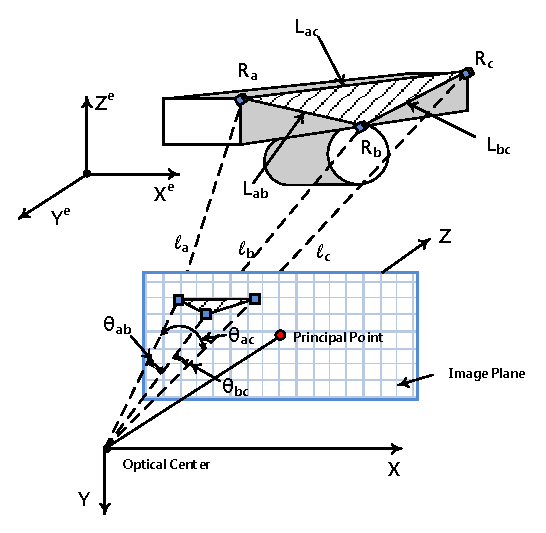
\includegraphics[width=1\linewidth, height=1.6in, clip,keepaspectratio]{ldp2cc.eps}
\caption{Determination of the location of user based on reference points.}\label{fig_ldp}
\end{figure}
We assume that the optical axis of the camera pierces the image plane on the \emph{principal point} and the \emph{focal length} of the camera is known.
As shown in Figure~\ref{fig_ldp}, the user takes a photo of the scene in front of him/her and three references points, namely, $R_a(X_a, Y_a, Z_a)$, $R_b(X_b, Y_b, Z_b)$ and $R_c(X_c, Y_c, Z_c)$ are projected to the image plane.
Through the reference point search scheme, we have obtained the correspondences between image points and reference points.
According to the distance from the image point projected by $R_a$ to the the point projected by $R_b$, we can easily derive $\theta_{ab}$, the angle between the line from the \emph{optical center} to $R_a$ and the line from the \emph{optical center} to $R_b$. We can also derive $\theta_{bc}$ and $\theta_{ac}$ in the same way.
%It has been proved that known the distances from three reference points to the \emph{optical center}, the location of the \emph{optical center} can be solved\cite{fischler1981random}.
% Thus the LDP problem can be transformed to the problem of calculating the distances from $n$ reference points to the optical center given locations of $n$ reference points as well as the angles from the optical center to each pair of reference points.
Let $L_{ab}$, $L_{bc}$ and $L_{ac}$ denote the distances between three reference points respectively, and $l_a$, $l_b$, $l_c$ denote the distances from each reference point to the \emph{optical center}.
We have the following equation group according to the law of cosine:
\begin{equation}
\label{equations}
\left\{
\begin{array}{l}
(L_{ab})^2 = (l_a)^2 + (l_b)^2 - 2 l_a\cdot l_b\cdot \cos(\theta_{ab})  \\
(L_{bc})^2 = (l_b)^2 + (l_c)^2 - 2 l_b\cdot l_c\cdot \cos(\theta_{bc}) \\
(L_{ac})^2 = (l_a)^2 + (l_c)^2 - 2 l_a\cdot l_c\cdot \cos(\theta_{ac})
\end{array}
\right.
\end{equation}
The above equation group may have multiple solutions,
%and after removing the geometrically isomorphic negative solutions, there are 4 solutions left.
we make use of the technique proposed in \cite{fischler1981random} to solve it and use the orientation of the camera to eliminate infeasible solutions. Every solution includes distances from three reference points to the \emph{optical center}.

We use the distance between query feature point and its nearest neighbor of reference point to measure the similarity of the match mentioned before. Each time, we select three matches with the highest similarity from the result set $T$ of that searching stage to form a trine.

Based on the solution of equation group~\ref{equations}, we are able to figure out the geographical location of the \emph{optical center} $CP(X,Y,Z)$, \ie user's geographical location, by solving another equation group~\ref{cp_equations}.
\begin{equation}
\label{cp_equations}
\left\{
\begin{array}{l}
\sqrt{(X-X_a)^2+(Y-Y_a)^2+(Z-Z_a)^2} = l_a  \\
\sqrt{(X-X_b)^2+(Y-Y_b)^2+(Z-Z_b)^2} = l_b \\
\sqrt{(X-X_c)^2+(Y-Y_c)^2+(Z-Z_c)^2} = l_c
\end{array}
\right.
\end{equation}
Equation group~\ref{cp_equations} describes the distances from $CP$ to three reference points. This equation group may have multiple solutions as well. Every solution will be treated without distinction to estimate its error.

We take the concept of "consensus" proposed by \cite{fischler1981random} to estimate error of each solution. With respect to the solution $S_0$, one reference point $r$ from $T$ reaches a consensus with $S_0$ if $r$ passes the estimate check function $Func$. $Func$ can be designed in a variety of forms. Our estimate check function $Func1$ is designed as follows: $Func1$ computes reference point $r$'s pixel coordinates in the picture which takes $S_0$ as the optical center. If the distance between $r$'s newly computed coordinates and its original coordinates does not exceed threshold $t$, then $r$ reaches a consensus with $S_0$. We put reference points which reach consensus with $S_0$ into consensus set $C_{S_0}$. If the ratio $\frac{|C_{S_0}|}{|T|}$ exceeds the threshold $w$, then $S_0$ will be considered as one candidate solution and added to set $F$. After every solution has been processed, we are able to figure out the final result of CP's location from set $F$ by selecting the candidate with highest consensus.
\subsection{Optimization of Estimate Check Function}
Aiming at enhancing localization performance of $Func1$, we refine it to form another estimate check function $Func2$ by appending a post-process after $Func1$. When we obtain $F$, rather than taking the candidate with highest consensus as the final result, we select the candidate through the vote. For one candidate $c$, a reference point $r$ in $T$ will vote for $c$ if the distance from $r$ to $c$ is not longer than threshold $d_{th}$. We discard the candidates with fewer votes and keep $K$ candidates with more votes. From these $K$ candidates, we pick the one derived from the trine whose triangle area is the largest among them as the final result.

$Func2$'s post-process is inspired by this phenomena: if three reference points in one trine are close to each other, then the solution of Equation group~\ref{equations} is more prone to error. If a trine has a larger area, the distances between three reference points in it are comparatively longer, which reduces the chance of error prone.

%When more reference points are observed, we compute the location of a user with different group of reference points and conduct an integrated optimization process to eliminate errors.
%In this work, we apply the Random Sample Consensus (RANSAC) \cite{fischler1981random} in our approach.
%RANSAC is an efficient method for fitting a model to experimental data. At the very beginning, it randomly select a minimum set of data points $S_1$ to instantiate the model $M_1$. Then RANSAC use $M_1$ to find the subset $S^c$ of data that are within some error bound. The subset is referred to as the \emph{consensus set} of $S_1$. If the number of $S^c$ is above some threshold, use $S^c$ to compute a new model. Otherwise, we select a new initiate set $S_2$ and repeat the above operations. This process ends after a number of rounds, we solve the problem with the largest consensus set. \mynote{check in paper}
%Our inverse localization scheme takes three types of inputs.

%\begin{enumerate}
%\item 1) A set of 5-tuples each of which includes the 3-D coordinates in earth coordinate system of a reference point, the 2-D image plane coordinated of the associated image point.
%\item 2) The probability $\omega$ that a 5-tuples contains a gross error.
%\item 3)
%\end{enumerate}

%The integrated algorithm contains the following steps.

%\begin{enumerate}
%\item 1) Three 5-tuples are selected and form the initial set $S1$.
%\item 2) The location of the optical center and thus the user is calculated accordingly.
%\item 3) Perturbing the image plane coordinated.
%\item 4) Perturbing the image plane coordinated.
%\end{enumerate}


%
%
%\subsection{Trace-based Optimization}
%Although our perspective approach calculate user locations based on data fusion from multiple reference points in the largest consensus set, the result at single location would still deviate from the real value or exhibits ambiguities while working under indistinctive indoor environments.
%It is due to the occasional ambiguities in vision feature matching. To address the problem, we present a trace-based algorithm to optimize the localization results. As users walk in the indoor environment, the localization service continuously generates locations at different points according to vision features. Besides, we can track the movement vectors of users using onboard sensors of the smart phone.
%A series of consecutive movement vectors form a trace that can connect successive localization snapshots.
%Based on the movement trace of a user, we can eliminate ambiguities and recover missing points by interpolation for the localization results.
%As shown in Figure~\ref{fig_trace}, for each pair of neighboring locations, we compute the similarity between the move vector and distance vector of the two locations. If the similarity of the two vectors are above a pre-specified threshold, these two locations are grouped into one component. Two adjacent components can merge to one. By this way, we find outliers among the locations. In the example of Figure~\ref{fig_trace}, with the movement vector, we can easily distinguish the correct location from the wrong ones.
%\begin{figure}[t!]
%\centering
%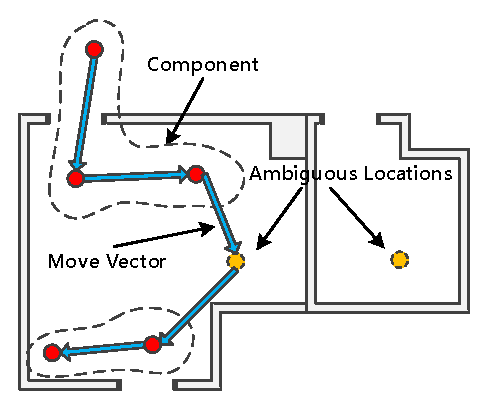
\includegraphics[width=1\linewidth, clip,keepaspectratio]{trace2.eps}
%\caption{Trace-based Optimization.}\label{fig_trace}
%\end{figure}
%Besides, the movement trace can also help us to recover missing coordinates by interpolation for the localization results.
%
%
%To obtain the moving vector of users, we apply one of the recent method proposed in Montage \cite{zhang2014montage} which combines dead reckoning and the stride length based approach to estimate the moving distance and leverage the filtered horizontal accelerations along the east and north axes at the earth coordinate system to measure the moving orientation of each step.
%
